\documentclass[a4paper, titlepage, 10pt]{report}
\usepackage[utf8]{inputenc}

\usepackage[magyar]{babel}
\usepackage[T1]{fontenc}

\usepackage{graphicx}
\usepackage{datetime}
\usepackage{hyperref}
\usepackage{url}
\usepackage{listings}
\usepackage[dvipsnames]{xcolor}
\usepackage{float} % kep környezetben H használatához (erősebb a h!-nél)
% https://stackoverflow.com/questions/2193307/how-do-i-get-latex-to-hyphenate-a-word-that-contains-a-dash
\usepackage[shortcuts]{extdash} % ``activity-implementációjának`` helyes elválasztásához
\usepackage{tocbibind} % irodalomjegyzék, tárgymutató a tartalomjegyzékbe
\usepackage[toc]{glossaries}
\usepackage{makeidx}
\usepackage{tikz}

\makeglossaries
\usetikzlibrary{shapes,calc,positioning}
\makeindex

% beszúr egy képet képaláírással és címkével
\newcommand{\kep}[4][1] { % a scale alapértelmezetten 1
	\begin{figure}[H]
		\centering \includegraphics[keepaspectratio, scale=#1]{#2}
		\caption{\centering #3}
		\label{fig:#4}
	\end{figure}
}

% https://github.com/cansik/kotlin-latex-listing
\lstdefinelanguage{Kotlin}{
  comment=[l]{//},
  commentstyle={\color{gray}\ttfamily},
  emph={filter, first, firstOrNull, forEach, lazy, map, mapNotNull, println},
  emphstyle={\color{OrangeRed}},
  identifierstyle=\color{black},
  keywords={!in, !is, abstract, actual, annotation, as, as?, break, by, catch, class,
	companion, const, constructor, continue, crossinline, data, delegate, do, dynamic,
	else, enum, expect, external, false, field, file, final, finally, for, fun, get, if,
	import, in, infix, init, inline, inner, interface, internal, is, lateinit, noinline,
	null, object, open, operator, out, override, package, param, private, property, protected,
	public, receiveris, reified, return, return@, sealed, set, setparam, super, suspend,
	tailrec, this, throw, true, try, typealias, typeof, val, var, vararg, when, where, while},
  keywordstyle={\color{NavyBlue}\bfseries},
  morecomment=[s]{/*}{*/},
  morestring=[b]",
  morestring=[s]{"""*}{*"""},
  ndkeywords={@Deprecated, @JvmField, @JvmName, @JvmOverloads, @JvmStatic, @JvmSynthetic,
	Array, Byte, Double, Float, Int, Integer, Iterable, Long, Runnable, Short, String, Any,
	Unit, Nothing, Activity},
  ndkeywordstyle={\color{BurntOrange}\bfseries},
  sensitive=true,
  stringstyle={\color{ForestGreen}\ttfamily},
}


\newacronym{off}{OFF}{OpenFoodFacts}
\newacronym{obf}{OBF}{OpenBeautyFacts}
\newacronym{opff}{OPFF}{OpenPetFoodFacts}
\newacronym{api}{API}{Application Programming Interface}
\newacronym{ocr}{OCR}{Optical Character Recognition}

\begin{document}

	\pagenumbering{roman}
	\begin{titlepage}
	\begin{center}
		
\includegraphics[keepaspectratio, width=8cm]{include/BME1782.eps} \\
		\vspace{5mm}

		\large \textbf{Budapesti Műszaki és Gazdaságtudományi Egyetem} \\
		Villamosmérnöki és Informatikai Kar \\
		Irányítástechnika és Informatika Tanszék \\
		\vspace{3cm}
		\huge \textbf{Nyílt~forráskódú Android~alkalmazás közösségi~fejlesztése}  \\
		\vspace{1cm}
		\textsc{Témalaboratórium beszámoló} \\
		\vfill
		\Large Főglein Simon István \\ ZA0D8T \\
		\vspace{1.6cm}
		\large Konzulens: Dr. Somogyi Péter
		\vfill
		\newdate{keszult}{04}{12}{2022}
		\large \displaydate{keszult}
	\end{center}
\end{titlepage}


	\tableofcontents

	\newpage
	\begin{abstract}
		\addcontentsline{toc}{chapter}{\abstractname}
		\pagenumbering{alph}
		\thispagestyle{plain}
		A témalaboratóriumom során egy nyílt forráskódú Android alkalmazáshoz fejlesztettem
		egy töltőképernyő funkciót, hogy az az újabb, Android 12-t és újabbat futtató rendszereken
		is megfelelően működjön.
		Ehhez részletesen megismerkedtem az Android dokumentációjával, példakódokat néztem, többféle
		megoldást teszteltem. A munkám során betekintést nyertem a közösségi szoftverfejlesztésbe,
		és egy nagy, több, mint félmillió felhasználó eszközén futó program hatalmas kódbázisába.
	\end{abstract}
	\pagenumbering{arabic}
	\newpage

	\chapter{Bevezetés, célkitűzések}
Napjainkban egyre gyakrabban szembesülünk az egészséges életmód betartásának nehézségeivel.
A Témalaboratórium tárgy keretein belül olyan szoftverfejlesztési feladattal szerettem volna
foglalkozni, ami kapcsolódik a választott témához (orvosi informatika) és gyakorlati
jelentősége is van, a szoftver használatával megkönnyíthetjük, jobbá tehetjük a felhasználók életét.

Ebben az irányban elindulva, számos különböző projektet átnézve és a konzulensemmel egyeztetve
döntöttem úgy, hogy a félév során az \acrlong{off}\footnote{Weboldal: \url{https://hu.openfoodfacts.org/}}
Android alkalmazását\footnote{GitHub: \url{https://github.com/openfoodfacts/openfoodfacts-androidapp}} fogom fejleszteni.
Miután ez az elhatározás megszületett, igyekeztem olyan feladatot vállalni,
ami megfelel a tárgy követelményeinek, tehát kellő mértékű kihívást jelent
az implementációja, olyan részeket is tartalmaz, melyekkel új ismereteket szerezhetek, és mégis
belefér a tárgy szűkös időkeretébe. Ezeket a szempontokat szem előtt tartva böngésztem a
projekthez tartozó hibajelentéseket és egyéb felhasználói kéréseket, javaslatokat (ún. \textit{feature request}-eket).
Így bukkantam rá egy olyan hibajegyre (\textit{GitHub Issue}), amelyben az alkalmazás
töltőképernyőjének (Splash screen) akkori implementációjának módosítását kérték, hogy
az Android 31-es API szint feletti, azaz Android 12-t vagy annál újabbat futtató eszközökön
is helyesen működjön.

Mivel korábban az egyetemen már volt lehetőségem betekintést nyerni a mobilos szoftverfejlesztésbe,
és régebbi Android verziót futtató készülékekhez már készítettem hasonló töltőképernyőt, továbbá
sok alkalmazásnál használnak ilyen megoldást, érdekelt, hogy miben újították meg a fejlesztés
folyamatát az új API bevezetésével.

A félév során tehát szerettem volna kipróbálni magam egy éles projektben, közelebbről megismerkedni
az Androidos szoftverfejlesztéssel, továbbá bővíteni Kotlin nyelvű ismereteimet.

	\chapter{Az OpenFoodFacts projekt rövid áttekintése}

Az \acrlong{off} egy közösségi kezdeményezés, mely arra irányul, hogy minél több ember
tájékozódhasson könnyen az élelmiszerek számos lényeges paraméteréről, így támogatva a
tudatos étkezést. Az alkalmazás segítségével több, mint másfél millió élelmiszerről kaphatunk
információt. Az ezekről elérhető fontosabb tulajdonságok a teljesség igénye nélkül:
\begin{itemize}
 \item Összetevők
 \item Allergén információk
 \item Tápérték adatok
 \item Nutri-score\footnote{Részletek a Nutri-score-ról: \url{https://hu.openfoodfacts.org/nutriscore}}
 \item Környezetre gyakorolt hatás, ökolábnyom
 \item Feldolgozottsági szint
\end{itemize}


Az alkalmazásban elérhető információk többségét a felhasználók maguk tölthetik fel az oldalra.
Ehhez használhatják például az \acrlong{off} applikációt az okostelefonjukon, melynek segítségével
beolvashatják egy adott élelmiszer vonalkódját, fotót készíthetnek a termékről, majd megadhatnak róla számtalan
részletet. A program támogatja az optikai szövegfelismerést (\acrfull{ocr}),
így akár a felhasználó időigényes közreműködése nélkül is ki tud nyerni lényeges információkat a
feltöltött képekből (\ref{fig:nutriextractionflow} ábra). Az így felvett információk bekerülnek egy adatbázisba, lehetővé téve a program többi
felhasználója számára az adatokhoz való szabad hozzáférést.
\kep[0.044]{include/nutrifacts-extraction.png}{Az \acrlong{off} képes automatikusan is információkinyerésre a feltöltött képek alapján. Forrás: \cite{autodataextraction}}{nutriextractionflow}

Az \acrlong{off} natív Android és iOS applikáció mellett rendelkezik egy keresztplatformos,
Flutter-alapú alkalmazással\footnote{\url{https://github.com/openfoodfacts/smooth-app}} is, továbbá egy webes alkalmazáson keresztül is hozzáférhetünk az
élelmiszerek adataihoz. A kliensek REST~API segítségével kommunikálhatnak a % TODO: rest api szójegyzékbe
szerverrel. Az \acrlong{off} architektúrájának sematikus rajza \az{\ref{fig:offarchitektura}}
ábrán látható. A továbbiakban az architektúra szerver oldali komponenseivel nem foglalkozom bővebben, az
ábrán kékkel jelölt mobilos kliensek közül is csak a natív Androidos alkalmazást mutatom be részletesebben.

% tikz ábra beszúrása
\begin{figure}[ht]
\centering
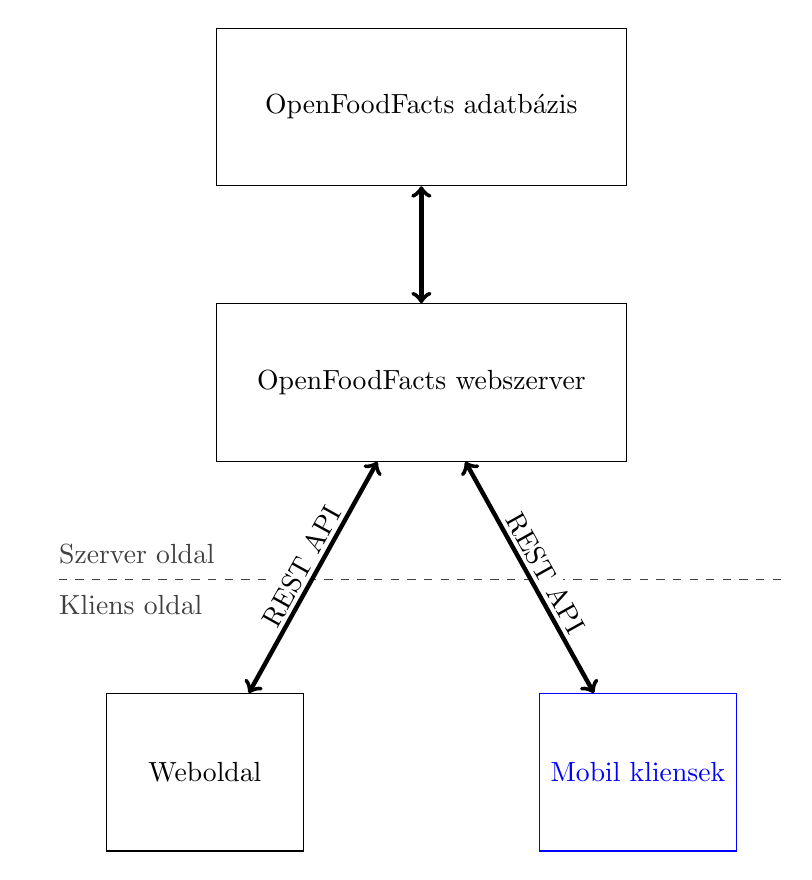
\begin{tikzpicture}[node distance=5cm and 1cm] \label{offarchitektura}
    \begin{scope}
        \node[shape=rectangle,draw,color=black, minimum height=2cm, minimum width=5.2cm] (OFFdb) { OpenFoodFacts adatbázis };
        \node[shape=rectangle, draw, color=black, minimum height=2cm, minimum width=5.2cm, yshift=1.5cm] (OFFwebsrv) [below of = OFFdb] { OpenFoodFacts webszerver };
            \begin{scope}[node distance=7cm]
                \node[shape=rectangle, draw, color=black, minimum height=2cm, minimum width=2.5cm, xshift=2.2cm] (OFFwebsite) [below left of = OFFwebsrv] { Weboldal };
                \node[shape=rectangle, draw, color=blue, minimum height=2cm, minimum width=2.5cm, xshift=-2.2cm] (mobileclients) [below right of = OFFwebsrv] { Mobil kliensek };
            \end{scope}
    \end{scope}
    \begin{scope}
        \path [clip] (-5,-8) rectangle (-1.88,-5) (-1.4,-8) rectangle (1.4,-5) (1.8,-8) rectangle (4.6,-5);
        \draw[darkgray, dashed] ([sloped, xshift=-2cm, yshift=-2.5cm]OFFwebsrv.west) to node [text width=3cm, anchor=west, above, xshift=-3.1cm, yshift=0.075cm] {Szerver oldal} node [text width=3cm, anchor=west, below, xshift=-3.1cm, yshift=-0.075cm] {Kliens oldal} ([sloped, pos=0.5, xshift=2cm, yshift=-2.5cm]OFFwebsrv.east);
    \end{scope}
    \draw[<->, ultra thick] (OFFdb) to node [sloped, pos=0.5, xshift=0.05cm, yshift=0.2cm] {} (OFFwebsrv);
    \draw[<->, ultra thick] (OFFwebsrv) to node [sloped, pos=0.5, xshift=0.05cm, yshift=0.2cm] {REST API} (OFFwebsite);
    \draw[<->, ultra thick] (OFFwebsrv) to node [sloped, pos=0.5, xshift=0.05cm, yshift=0.2cm] {REST API} (mobileclients);
\end{tikzpicture}

\caption{\centering Az \acrlong{off} rendszer architektúrája, a mobilos kliensek elhelyezkedése az architektúrában}
\label{fig:offarchitektura}
\end{figure}

	\chapter{Androidos SplashScreen megoldások ismertetése}
\section{API level 30 (Android 11) és korábbi}
Az Android 12-ben bevezetett új API előtt nem volt rendszerszintű támogatás töltőképernyők
fejlesztésére, így a fejlesztők két lehetőség közül választhattak: % TODO: forrás: https://developer.android.com/develop/ui/views/launch/splash-screen/migrate
\begin{itemize}
 \item Egyedi téma bevezetése, amivel a nézet \textit{windowBackground} propertyjét változtatták meg,
 majd állították vissza az alkalmazás betöltését követően az alapértelmezett értékre
 \item Egyedi \textit{Activity} létrehozásával: ezzel egy dedikált osztályt és nézetet hozunk létre
 a töltőképernyő funkció megvalósítására, amely a betöltést vagy timeoutot követően elindítja
 az alkalmazás főképernyőjét % TODO: explicit intenttel, de erre nem biztos, hogy ebben a fejezetben ki kell térni
 % TODO: api a rövidítésjegyzékbe
 % TODO: timeout a szójegyzékbe
 % TODO: Activity a szójegyzékbe: ``An activity is a single, focused thing that the user can do. Almost all activities interact with the user, so the Activity class takes care of creating a window for you in which you can place your UI with''
 %          Forrás: https://developer.android.com/reference/android/app/Activity
\end{itemize}


Az OpenFoodFacts alkalmazásban az utóbbit választották a fejlesztők, ez viszont azt eredményezte,
hogy Android 11 fölötti eszközökön két különböző töltőképernyő jelent meg az alkalmazás indulásakor,
emiatt vált szükségessé az alkalmazás felkészítése az újabb verzióval való helyes működésre.

\section{API level 31 (Android 12) és újabb}
A SplashScreen API bevezetésével maga az operációs rendszer biztosít egységes megoldást
töltőképernyő készítésére. Ez olyan lehetőségekkel bővítette a programozók eszköztárát, ami korábban
nem, vagy csak körülményesen volt megvalósítható (pl. animált ikonok beállítása
a töltőképernyőre).
Az új API arra is lehetőséget ad, hogy a régebbi szoftververziót futtató eszközökön a SplashScreen
compat könyvtár % TODO: app compat hivatkozása
segítségével biztosítsuk a visszafele kompatibilitást.

	\chapter{Jelentősebb állomások a~fejlesztés során}
Munkám jelentős részét az Android dokumentációjának tanulmányozása, illetve a különböző lehetőségek
tesztelése tette ki. Fontos volt még megismerni a projekt fejlesztésére vonatkozó irányelveket
(pl. kódformázási konvenciók, pull requestek pontos leírása).

\section{Ismerkedés a projekttel}
A projekt meghatározását követően igyekeztem megismerni annak felépítését, kideríteni, hogy
pontosan melyik modulokkal kell majd dolgoznom a töltőképernyő frissebb verziójának elkészítéséhez.
Ehhez klónoztam a projekt \gls{github} repositoryját, és az \gls{androidstudio} fejlesztőkörnyezet
segítségével részletesen tanulmányoztam a projekt struktúráját, a releváns kódrészleteket,
beszereztem a függőségeket, és lefordítottam a programot.

\section{Migrálás az új API-ra, visszafelé kompatibilitás biztosítása}
Android 12-es verziót futtató emulátor telepítését követően az Android fejlesztői
dokumentációjában fellelhető migrációs útmutatóból tájékozódtam a további feladataimról.
Az itt leírtakat követve a töltőképernyő helyesen jelent meg az \acrshort{api} 31-et futtató emulátoron.
Ilyen funkció esetében azonban nem feledkezhetünk meg a visszafelé kompatibilitás támogatásáról
sem, ezért szükséges volt az új \acrshort{api}-t nem ismerő eszközökön is tesztelni a megoldást.
A régebbi \acrshort{api} verziót futtató eszközök esetében azt a megoldást választottam, hogy a már meglévő
töltőképernyő jelenjen meg (azaz egy külön splash screen activity induljon el az alkalmazás
indulásakor), míg az újakon a frissen implementált verzió. A~funkció tesztelése során
megállapítottam, hogy a megoldás alapvetően az elvárt eredményt adja, azonban -- ahogy az a
\gls{github} issue-ban is szerepelt -- az éjszakai módban nem az elvárt módon működik: sötét helyett
fehér háttérszínnel jelenik meg a képernyő. A hibajegyhez mellékelt képernyőképen szereplőhöz
hasonló kinézetű töltőképernyőt az emulátoron nem sikerült reprodukálni, ott az éjszakai mód
bekapcsolását követően is fehér háttérszínnel indult el a töltőképernyő, csak az alkalmazás
további részei használták az éjszakai témát. Mivel Android 12-t futtató eszköz nem állt
rendelkezésemre, ezért valódi hardveren nem tudtam tesztelni a megoldást.

% TODO: megoldás szóismétlés
A heti munkám során alkalmam nyílt megismerni egy, az Androidos szoftverfejlesztésben elterjedt
megoldást az alkalmazás különböző verzióinak egyszerű előállítására. Ebben a projektben ez
különösképpen nagy jelentőséggel bír, mert nem csak arról van szó, hogy az alkalmast több
alkalmazásboltban is terjesztik (pl. Google Play, F-Droid), hanem ugyanarra a kódbázisra
három különböző alkalmazást (\acrfull{off}, \acrfull{obf}, \acrfull{opff})
is építenek. Ez azért is lehetséges, mert az alkalmazás lényegében csak egy felhasználói felület
az \acrlong{off} (és a többi verzió) adatbázisának elérésére. Így maga a kliens oldali alkalmazás
az ikonok és egyéb felhasználói elemek kivételével megegyezik a három verzió között.
A build variants % TODO ...

% Build variants: az OpenFoodFacts csapata az élelmiszerek mellett többféle termékkategóriához
% készít szoftvert (pl. szépészeti készítmények, állateledelek). Mivel mindezek a verziók szoftveresen
% nagyon hasonlóak, csak más-más backendet használnak, ezért mindössze egyetlen Android appot
% készítenek, melyet lehetőség van különféle verziókra (flavor) fordítani. Eleinte nehézséget okozott,
% hogy alapértelmezetten a git repository klónozását követően az OpenBeautyFacts alkalmazás
% települt. Mivel az alkalmazás szinte teljesen megegyezik az OpenFoodFacts alkalmazással, a
% tesztelés során ez nem jelentett gondot, de a splash screenen megjelenő ikon más, ezért az éjszakai
% mód teszteléséhez már az OpenFoodFacts-et volt szükséges telepíteni. Némi kutatómunka után
% találtam rá arra a lehetőségre Android Studioban, amivel a fordítandó build variant-ot lehet
% kiválasztani. Így a továbbiakban a Google Play-re targetelt OpenFoodFacts alkalmazással
% folytattam a fejlesztést.

% TODO: ez még szerkesztésre szorul, csak át lett emelve a második hét alfejezetből,
%       de ide való
\section{Implementáció továbbfejlesztése: éjszakai mód támogatása}
Ezen a héten a munkám az éjszakai módban látható töltőképernyő helyes megjelenítésére irányult.
Sikerült kölcsönkérnem egy Android 12-es verziót futtató eszközt, azonban ezen sem sikerült
előállítanom a \gls{github} issue-ban szereplő módon a hibát, így folytattam a hiba okának felkutatását
a kódban és az interneten egyaránt. Rövid utánajárást követően kiderült, hogy a
\textit{styles.xml} fájlból nem volt megadva \textit{night} erőforrás-módosítóval
(resource modifier) ellátott verzió. Ezt a hiányosságot pótoltam, létrehoztam egy éjszakai
módban helyesen megjelenő stílus erőforrást. Ebben a háttérszín megváltoztatásán túl szükséges
volt a SplashScreen \acrshort{api}-által biztosított témából egy sajátot leszármaztatni, mely rendelkezik
az ikon helyes megjelenítéséhez szükséges propertykkel. Az így született \gls{tema} az alábbi:

\begin{lstlisting}[frame=single,language=xml,emph={style,item},
    emphstyle=\color{BurntOrange}\textbf,stringstyle=\color{OliveGreen}\textbf]
<style name="SplashTheme"
  parent="Theme.SplashScreen.IconBackground">
    <item name="windowSplashScreenBackground">
        @color/grey_800
    </item>
    <item name="windowSplashScreenIconBackgroundColor">
        @color/grey_400
    </item>
    <item name="postSplashScreenTheme">
        @style/Theme.AppCompat.DayNight
    </item>
    <item name="windowSplashScreenAnimatedIcon">
        @mipmap/ic_launcher_round
    </item>
</style>
\end{lstlisting}

Ez azonban nem jelentett megoldást, mert a \gls{tema}, amiből az \acrshort{api} 30 feletti helyes működésért
le kell származtatnunk a saját \glslink{tema}{témánkat}, nem támogatja az \gls{appcompat}\gls{activity} használatát, ami
az \acrlong{off} activity\-/implementációjának ősosztálya. Így a SplashScreen \acrshort{api} által biztosított
téma kizárólagos használatával az alkalmazás a töltőképernyő megjelenítését követően crashelt,
ez \az{\ref{fig:appcompatcrash}} ábrán látható.
\kep[0.5]{include/theme-appcompat-crash.png}{\textit{AppCompat} téma használata nélkül
az alkalmazás összeomlik}{appcompatcrash}

A probléma megoldására a StackOverflow-n és az Android fejlesztői oldalán elérhető leírás
nyújtott iránymutatást. A \textit{postSplashScreenTheme} property megfelelő beállítását követően
az alkalmazás már megfelelően működött, a töltőképernyő után a főképernyő helyesen jelent meg.
Így az éjszakai módban használt téma kódja az alábbi:

\begin{lstlisting}[frame=single,language=xml,emph={style,item},
    emphstyle=\color{BurntOrange}\textbf,stringstyle=\color{OliveGreen}\textbf]
 <style name="SplashTheme"
   parent="Theme.SplashScreen.IconBackground">
    <item name="windowSplashScreenBackground">
        @color/grey_800
    </item>
    <item name="windowSplashScreenIconBackgroundColor">
        @color/grey_400
    </item>
    <item name="postSplashScreenTheme">
        @style/Theme.AppCompat.DayNight
    </item>
</style>
\end{lstlisting}

A fent definiált téma az alábbi módon jelenik meg a gyakorlatban (\ref{fig:darktheme} ábra):
\kep[0.11]{include/darktheme.png}{A töltőképernyő éjszakai módban, Android 12-n}{darktheme}


\section{Egyezetés a projekt fejlesztőivel}
A negyedik héten kommunikációt folytattam az alkalmazás fejlesztőivel a pull request lehetséges
javításairól, illetve ennek merge-öléséről. Az alkalmazás egyik fejlesztője egy import
eltávolítását javasolta, rövid utánajárást követően \cite{extensionfunction} én viszont arra jutottam, hogy ez nem
hagyható el, ugyanis egy ún. Kotlin \textit{extension function}-ről van szó, amire az import
nélkül nem tudunk hivatkozni. A Kotlinban támogatott extension function-ök olyankor lehetnek
hasznosak, amikor egy már -- nem általunk -- megírt osztály lehetőségeit szeretnénk bővíteni.
Ilyen megoldást alkalmaztak a SplashScreen könyvtár fejlesztői is, az Android által biztosított
Activity osztályt bővítették ki egy \textit{installSplashScreen} metódussal:

\begin{lstlisting}[frame=single,language=Kotlin,emph={style,item}
    ,caption=Részlet a SplashScreen könyvtár kódjából az extension function-nel]
 public fun Activity.installSplashScreen():
            SplashScreen {
    // ...
 }
\end{lstlisting}
\kep[0.59]{include/gh-discussion.png}{Egyeztetés a projekt egyik fejlesztőjével az extension function importjáról}{ghdiscussion}

Végül a projekt másik fejlesztője is az enyémmel azonos következtetésre jutott, az import
nem hagyható el, így a módosításaim elfogadásra jutottak, és bekerültek az alkalmazás kódbázisába.

% TODO: backwards compatibility támogatása
%       sötét téma
%       https://developer.android.com/develop/ui/views/launch/splash-screen/migrate#best-practices
%       https://developer.android.com/reference/android/window/SplashScreen
%       https://developer.android.com/develop/ui/views/launch/splash-screen
%       https://github.com/openfoodfacts/openfoodfacts-androidapp/pull/4871
%       https://github.com/openfoodfacts/openfoodfacts-androidapp/issues/4548
%       https://kotlinlang.org/docs/extensions.html#scope-of-extensions
% GitHub fogalomjegyzékbe
% repository fogalomjegyzékbe
% Android Studio fogalomjegyzékbe
% emulátor fogalomjegyzékbe
% TODO: \begin{verbatim} helyett \begin{xmlcode}
% TODO: AppCompatActivity hivatkozása

	\chapter{Összegzés}

A Témalaboratórium tárgy keretein belül alkalmam nyílt betekintést nyerni egy élő,
aktívan fejlesztés alatt álló, széles felhasználói körrel rendelkező projekt fejlesztésébe.
Ezalatt számos új ismeretre tettem szert: ízelítőt kaptam, hogy hogyan lehet kiigazodni egy
összetett szoftver forrásfájljai között, hogyan lehetséges olyan emberekkel közösen dolgozni
egy ilyen kihíváson, akikkel sosem találkoztam, és több ezer kilométerre élnek tőlem.
Megtanultam továbbá, hogy hogyan lehetséges egy alkalmazás forráskódját más hasonló
szoftverben is újrafelhasználni, mi a különböző alkalmazásboltok és ezek sajátosságainak
kezelésének módja. Ezen kívül korábbi tapasztalataimat is bővítettem: jobban elmélyültem
a Kotlin nyelv által nyújtott eszközök, modern nyelvi elemek használatában
(pl. extension function-ök), lehetőségem volt szélesebb körben megismerkedni az Androidos
szoftverfejlesztéssel, valamint áthatóan megismertem néhány könyvtárat
(pl. \gls{splashscreen}, \gls{appcompat}).

A féléves munkám pedig a megszerzett tudáson túl is kifizetődött, ugyanis az álalam
készített töltőképernyő-implementáció bekerült az alkalmazás kódbázisába, így több
százezer felhasználó találkozhat vele nap mint nap a program indítása során.


	\printindex
	\printglossaries
	\bibliographystyle{plaindin}
	\bibliography{irodalomjegyzek}

\end{document}
